\documentclass[t]{beamer}
\usetheme[deutsch]{KIT}
\setbeamercovered{transparent}
\setbeamertemplate{navigation symbols}{}

\KITfoot{Tutoriumsmaterial von Alexander Kwiatkowski, Michael Vollmer und Matthias Holoch \hspace{2.5cm} Basierend auf den Folien von Simon Stroh und Moritz v. Looz}
\usepackage[utf8]{inputenc}
\usepackage{amsmath}
\usepackage{ifthen}
\usepackage{amssymb}
\usepackage{tikz}
\usepackage{ngerman}
\usepackage[normalem]{ulem}
\usetikzlibrary{automata}
\usenavigationsymbols


\title{Theoretische Grundlagen der Informatik}
\subtitle{Tutorium}
\author{Alexander Kwiatkowski, Michael Vollmer und Matthias Holoch}

\institute[IKS]{Institut für Kryptographie und Sicherheit}

\TitleImage[height=\titleimageht]{images/tmaschine.png}

\newcommand{\N}{\ensuremath{\mathbb{N}}}
\newcommand{\M}{\ensuremath{\mathcal{M}}}
\newcommand{\classP}{\ensuremath{\mathcal{P}}}
\newcommand{\classNP}{\ensuremath{\mathcal{NP}}}
\newcommand{\co}{\ensuremath{\mathsf{co\text{-}}}}
\newcommand{\pot}{\ensuremath{\mathcal{P}}}
\newcommand{\abs}[1]{\ensuremath{\left\vert #1 \right\vert}}
\newcommand{\menge}[2]{\ensuremath{\left\lbrace #1 \,\middle\vert\, #2 \right\rbrace}}
\newcommand{\ducttape}[1]{\vspace{#1}}
\newcommand{\neglit}[1]{\overline{#1\vphantom{x^a}}}
\newcommand{\recipe}{\raisebox{-.3cm}{
\includegraphics[scale=.15]{images/chefs-cap.png}}\hspace{0.2cm}}
\newcommand{\opt}[1]{\ensuremath{\text{OPT}(#1)}}
\newcommand{\A}[1]{\ensuremath{\mathcal{A}(#1)}}
\renewcommand{\O}[1]{\ensuremath{\mathcal{O}(#1)}}
\newcommand{\msout}[1]{\text{\sout{\ensuremath{#1}}}}

\newcommand{\invincible}{\setbeamercovered{invisible}} %  "Yesss! I am invincible!!" (Boris Grishenko)
\newcommand{\vincible}{\setbeamercovered{transparent}}
\renewcommand{\solution}[1]{\invincible \pause #1 \vincible}
\newcommand{\micropause}{\\[8pt]}

% \@ifundefined{tikzset}{}{\tikzset{initial text=}} % Text "start" bei Startknoten unterdrücken
\tikzstyle{every node}=[thick]
\tikzstyle{every line}=[thick]

\newcommand{\tutnr}[1]{
  \subtitle{Tutorium #1}
	\begin{frame}
		\maketitle
	\end{frame}
}

\newcommand{\uebnr}[1]{
  \subtitle{Anmerkungen zum #1. Übungsblatt}
	\begin{frame}
		\maketitle
	\end{frame}
}

\begin{document}

\newcommand{\start}[3]
{
  \draw (#1*2,#2*2) node{$#3$};
  \draw (#1*2,#2*2) circle(0.4cm);
  \draw [->] (#1*2-0.9,#2) -- (#1*2-0.4,#2);
}
\newcommand{\final}[3]
{
  \draw (#1*2,#2*2) node{$#3$};
  \draw (#1*2,#2*2) circle(0.4cm);
  \draw (#1*2,#2*2) circle(0.32cm);
}
\newcommand{\startfinal}[3]
{
  \draw (#1*2,#2*2) node{$#3$};
  \draw (#1*2,#2*2) circle(0.4cm);
  \draw (#1*2,#2*2) circle(0.32cm);
  \draw [->] (#1*2-0.9,#2) -- (#1*2-0.4,#2);
}
\newcommand{\state}[3]
{
  \draw (#1*2,#2*2) node{$#3$};
  \draw (#1*2,#2*2) circle(0.4cm);
}
\newcommand{\tol}[4]
{
  \draw (#1+#3,#2*2) node[above]{$#4$};
  \draw [->] (#1*2-0.4,#2*2) -- (#3*2+0.4,#2*2);
}
\newcommand{\tor}[4]
{
  \draw (#1+#3,#2*2) node[above]{$#4$};
  \draw [->] (#1*2+0.4,#2*2) -- (#3*2-0.4,#2*2);
}
\newcommand{\tot}[4]
{
  \draw (#1*2,#2+#3) node[right]{$#4$};
  \draw [->] (#1*2,#2*2+0.4) -- (#1*2,#3*2-0.4);
}
\newcommand{\tob}[4]
{
  \draw (#1*2,#2+#3) node[right]{$#4$};
  \draw [->] (#1*2,#2*2-0.4) -- (#1*2,#3*2+0.4);
}
\newcommand{\totl}[5]
{
  \draw (#1+#3,#2+#4) node[above right]{$#5$};
  \draw [->] (#1*2-0.283,#2*2+0.283) -- (#3*2+0.283,#4*2-0.283);
}
\newcommand{\totr}[5]
{
  \draw (#1+#3,#2+#4) node[above left]{$#5$};
  \draw [->] (#1*2+0.283,#2*2+0.283) -- (#3*2-0.283,#4*2-0.283);
}
\newcommand{\tobl}[5]
{
  \draw (#1+#3,#2+#4) node[below right]{$#5$};
  \draw [->] (#1*2-0.283,#2*2-0.283) -- (#3*2+0.283,#4*2+0.283);
}
\newcommand{\tobr}[5]
{
  \draw (#1+#3,#2+#4) node[below left]{$#5$};
  \draw [->] (#1*2+0.283,#2*2-0.283) -- (#3*2-0.283,#4*2+0.283);
}
\newcommand{\rloopl}[3]
{
  \draw (#1*2-1,#2*2) node[left]{$#3$};
  \draw [->] (#1*2-0.35,#2*2-0.2) arc (-30:-320:0.32cm);
}
\newcommand{\rloopr}[3]
{
  \draw (#1*2+1,#2*2) node[right]{$#3$};
  \draw [->] (#1*2+0.35,#2*2+0.2) arc (150:-140:0.32cm);
}
\newcommand{\rloopt}[3]
{
  \draw (#1*2,#2*2+1) node[above]{$#3$};
  \draw [->] (#1*2-0.2,#2*2+0.35) arc (240:-50:0.32cm);
}
\newcommand{\rloopb}[3]
{
  \draw (#1*2,#2*2-1) node[below]{$#3$};
  \draw [->] (#1*2+0.2,#2*2-0.35) arc (60:-230:0.32cm);
}
\newcommand{\lloopl}[3]
{
  \draw (#1*2-1,#2*2) node[left]{$#3$};
  \draw [->] (#1*2-0.35,#2*2+0.2) arc (30:320:0.32cm);
}
\newcommand{\lloopr}[3]
{
  \draw (#1*2+1,#2*2) node[right]{$#3$};
  \draw [->] (#1*2+0.35,#2*2-0.2) arc (-150:140:0.32cm);
}
\newcommand{\lloopt}[3]
{
  \draw (#1*2,#2*2+1) node[above]{$#3$};
  \draw [->] (#1*2+0.2,#2*2+0.35) arc (-60:230:0.32cm);
}
\newcommand{\lloopb}[3]
{
  \draw (#1*2,#2*2-1) node[below]{$#3$};
  \draw [->] (#1*2-0.2,#2*2-0.35) arc (-240:50:0.32cm);
}
\include{amsmath}
\tutnr{6}

\section{Gödelnummer}
\subsection{Gödelnummer Erklärung}
\begin{frame}
	\frametitle{Gödelnummer}
	\begin{itemize}
		\item Jede Turingmaschine lässt sich eindeutig als natürliche Zahl darstellen. \\ Diese Zahl ist ihre \emph{Gödelnummer}.
		\begin{itemize}
			\item Das bedeutet auch, dass die Menge aller Turingmaschinen abzählbar ist!
		\end{itemize}
		\item Eine Möglichkeit eine Turingmaschine binär zu kodieren wäre folgende: \\
		Alle $n$ Zustandsübergänge $\delta(q_i, x_j) = (q_k, x_l, d_m)$, \\
		mit $d_1 = L$, $d_2 = N$, $d_3 = R$ \\
		kodieren in \\
		$111 code_1 11 code_2 11 ... 11 code_{n-1} 11 code_n 111$ \\
		Wobei $code_r$ so kodiert ist: \\
		$0^i 1 0^j 1 0^k 1 0^l 1 0^m$
		\item Eine solche eindeutige Kodierung nennen wir \emph{Gödelisierung}.
	\end{itemize}
\end{frame}

\begin{frame}
	\frametitle{Universelle Turingmaschine}
\begin{itemize}
	\item Eingabe:
	\begin{enumerate}
	\item Kodierung einer TM
	\item Eingabe für die zu simulierende TM
	\end{enumerate}
	\item Simulation der übergebenen TM
	\item Ausgabe: Ausgabe der simulierten TM.
	\end{itemize}
\end{frame}
\section{Entscheidbarkeit}
\subsection{Erklärung}
\begin{frame}
	\frametitle{Definitionen zur Entscheidbarkeit}
	 \begin{enumerate}
  \item Eine TM \emph{akzeptiert} eine Eingabe $w \in \Sigma^*$, wenn sie nach Lesen von $w$ im akzeptierenden Zustand stoppt.
  \item Sie \emph{akzeptiert} eine Sprache $L \subseteq \Sigma^*$, wenn sie genau die Wörter $w$ aus $L$ als Eingabe akzeptiert.
  \item Eine Sprache $L \subseteq \Sigma^*$ heißt \emph{rekursiv} oder \emph{entscheidbar}, wenn es eine Turingmaschine gibt, die auf allen Eingaben stoppt und
	ein Wort $w \in \Sigma^*$ genau dann akzeptiert, wenn $w \in L$ gilt.
\end{enumerate}
\end{frame}
\begin{frame}
	\frametitle{Definitionen zur Entscheidbarkeit}
 \begin{enumerate}
 \setcounter{enumi}{3}
  \item Eine Sprache $L \subseteq \Sigma^*$ heißt \emph{rekursiv-aufzählbar} oder \emph{semi-entscheidbar}, wenn es eine Turingmaschine gibt, die ein Wort $w \in \Sigma^*$ genau dann akzeptiert, wenn $w \in L$ gilt. \\ Das Verhalten der Turingmaschine für Eingaben $w \not\in L$ ist damit nicht definiert.
	Sie stoppt entweder nicht in einem Endzustand oder aber stoppt gar nicht.
	\item Eine TM \emph{realisiert} die Funktion $f: \Sigma^* \rightarrow \Gamma^*$ mit $$f(w) = \begin{cases} \text{Ausgabe der TM nach Abarbeitung von } w & \text{wenn die TM hält} \\ \text{undefiniert} & \text{sonst} \end{cases}$$
 \end{enumerate}
\end{frame}
\subsection{Halteproblem}
\begin{frame}
	\frametitle{Halteproblem}
	Das Halteproblem beschreibt die Aufgabe zu entscheiden, ob eine Turingmaschine bei gegeben Eingabewort hält oder nicht. Dieses Problem ist im allgemeinen Fall semi-entscheidbar, aber nicht entscheidbar.
\end{frame}
\subsection{Beispiel B5 A4}
\begin{frame}
	\frametitle{Beispielaufgabe Entscheidbarkeit (B5 A4)}
	Zeigen Sie, dass die Sprache \\ $\mathcal{L} = \{ \langle \mathcal{M} \rangle \; | \; \mbox{Turingmaschine $\mathcal{M}$ akzeptiert jede Eingabe} \}$ \\ nicht entscheidbar ist!
\end{frame}
\subsection{Aufgabe B6 A1}
\begin{frame}
	\frametitle{Aufgabe B6 A1}
	Zeigen Sie, dass die Sprache \\ $\mathcal{L} = \{\langle\mathcal{M}\rangle \; | \; \mbox{Turingmaschine $\mathcal{M}$ hat mindestens einen unerreichbaren Zustand}\}$ \\ nicht entscheidbar ist!
\end{frame}

\section{Postsches Korrespondenzproblem}
\subsection{Erklärung}
\section{Postsches Korrespondenzproblem}
\subsection{Postsches Korrespondenzproblem}
\begin{frame}
\frametitle{Postsches Korrespondenzproblem}
Gegeben sei eine Folge $P$ von Paaren $((x_1, y_1), (x_2, y_2), \ldots, (x_n,y_n))$ von nichtleeren Worten über einem endlichen Alphabet. Dies nennt man eine \textbf{Instanz} des PKP.
Eine nichtleere Folge $I = i_1, i_2, \ldots, i_m$ von Indizes aus $\{1, \ldots, n\}$ heißt Lösung zu $P$, wenn $x_{i_1}x_{i_2}\ldots{}x_{i_m} = y_{i_1}y_{i_2}\ldots{}y_{i_m}$.
\only<2->{\begin{block}{Beispiel}
\begin{displaymath}
( {a \choose aba}, {ab \choose bb}, {baa \choose aa} )
\end{displaymath}

\only<3>{Lösung: $1,3,2,3$
\begin{displaymath}
{a \choose aba}, {baa \choose aa}, {ab \choose bb}, {baa \choose aa}
\end{displaymath}}

\end{block}}
\end{frame}
\subsection{Aufgabe B5 A2}
\begin{frame}
	\frametitle{Aufgabe B5 A2}
	Geben Sie, sofern m"oglich, je eine L"osung f"ur die folgenden Post-Systeme an! \\
	Begr"unden Sie gegebenenfalls, warum es keine L"osung geben kann!
	\vspace{5mm}
	\begin{enumerate}
		\item \begin{displaymath} \{ {aa \choose a}, {b \choose aa}, {a \choose aab} \} \end{displaymath}
		\item \begin{displaymath} \{ {01 \choose 0}, {0 \choose 101}, {101 \choose 0} \} \end{displaymath}
	\end{enumerate}
\end{frame}

\subsection{Troll-Aufgabe}
\begin{frame}
\frametitle{Aufgabe}
Finde eine Lösung für folgende Instanz des PKP:
$$ ((001,0),(01,011),(01,101),(10,001)) $$

\invincible
\pause

Eine kürzeste Lösung hat mindestens die Länge 66, z.B:
\begin{center}
$ I_1 = (2, 4, 3, 4, 4, 2, 1, 2, 4, 3, 4, 3, 4, 4, 3, 4, 4, 2, 1, 4,$ \\
$4, 2, 1, 3, 4, 1, 1, 3, 4, 4, 4, 2, 1, 2, 1, 1, 1, 3, 4, 3, 4, 1, 2,$ \\
$1, 4, 4, 2, 1, 4, 1, 1, 3, 4, 1, 1, 3, 1, 1, 3, 1, 2, 1, 4, 1, 1, 3)$
\end{center}

\pause


\includegraphics{images/trollface}

\vincible

\end{frame}

\section{Mehr Übungsaufgaben}
\subsection{Aufgabe B6 A4}
\begin{frame}
	\frametitle{Aufgabe B6 A4 Entscheidbarkeit}
	Sei $A \subseteq \mathbb{N}_0$ eine entscheidbare Menge. \\
	Zeigen Sie, dass $ B := \{x+2y^2+17+11^x \; | \; x,y \in A\}$ entscheidbar ist!
\end{frame}
\subsection{Aufgabe B6 A3}
\begin{frame}
	\frametitle{Aufgabe B6 A3 rekursiv aufzählbare Mengen}
	Welche der folgenden Mengen sind rekursiv aufz"ahlbar? \\
	Beweisen Sie Ihre Aussage!
	\begin{enumerate}
		\item $M_1 := \{q \in \mathbb{Q} \; | \; 0<q<1\}$
		\item $M_2 := \{r \in \mathbb{R} \; | \; 0<r<1\}$
	\end{enumerate}
\end{frame}

\section{Schluss}
\subsection{Schluss}
\begin{frame}
\frametitle{Bis zum nächsten Mal!}
\begin{center}
  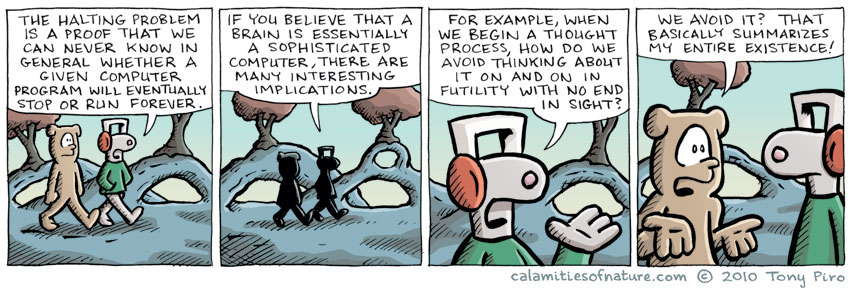
\includegraphics[width=1.59 \textheight]{images/halting.jpg}
\end{center}
\end{frame}

\frame{
  \frametitle{Lizenzen}
  \center
  
\includegraphics[width=2em]{images/by}
  
\includegraphics[width=2em]{images/cc}
  
\includegraphics[width=2em]{images/sa}
  \\
  {\tiny

Dieses Werk ist unter einem ``Creative Commons Namensnennung-Weitergabe unter gleichen Bedingungen 3.0 Deutschland``-Lizenzvertrag lizenziert. Um eine Kopie der Lizenz zu erhalten, gehen Sie bitte zu \href{http://creativecommons.org/licenses/by-sa/3.0/de/}{http://creativecommons.org/licenses/by-sa/3.0/de/} oder schreiben Sie an Creative Commons, 171 Second Street, Suite 300, San Francisco, California 94105, USA.\\
  \vspace{1cm}
  Davon ausgenommen sind das Titelbild, welches aus der März-April 2002 Ausgabe von American Scientist erschienen ist und ohne Erlaubnis verwendet wird, sowie das KIT Beamer Theme. Hierfür gelten die Bestimmungen der jeweiligen Urheber.
  \vspace{1cm}
  \\ 
  }
  %Habe hier die Reihenfolge etwas umgestellt, weil die Formatierung bei mir komisch aussah. 
  %Wenn es bei dir anders ist, kannst du es auch wieder zurückändern, dann haben wir unterschiedliche Kompilieroptionen
}

\end{document}